\clearpage
\subsection{Development Tools}
In Embedded linux development it is common to use any text editor with code syntax highlighting.
This project uses \verb|VSCode| as its development platform.

For compiling the \verb|C++| code it uses \verb|CMake| with the following \verb|CMakeLists.txt| file.

\begin{figure}[!htb]
    \centering
    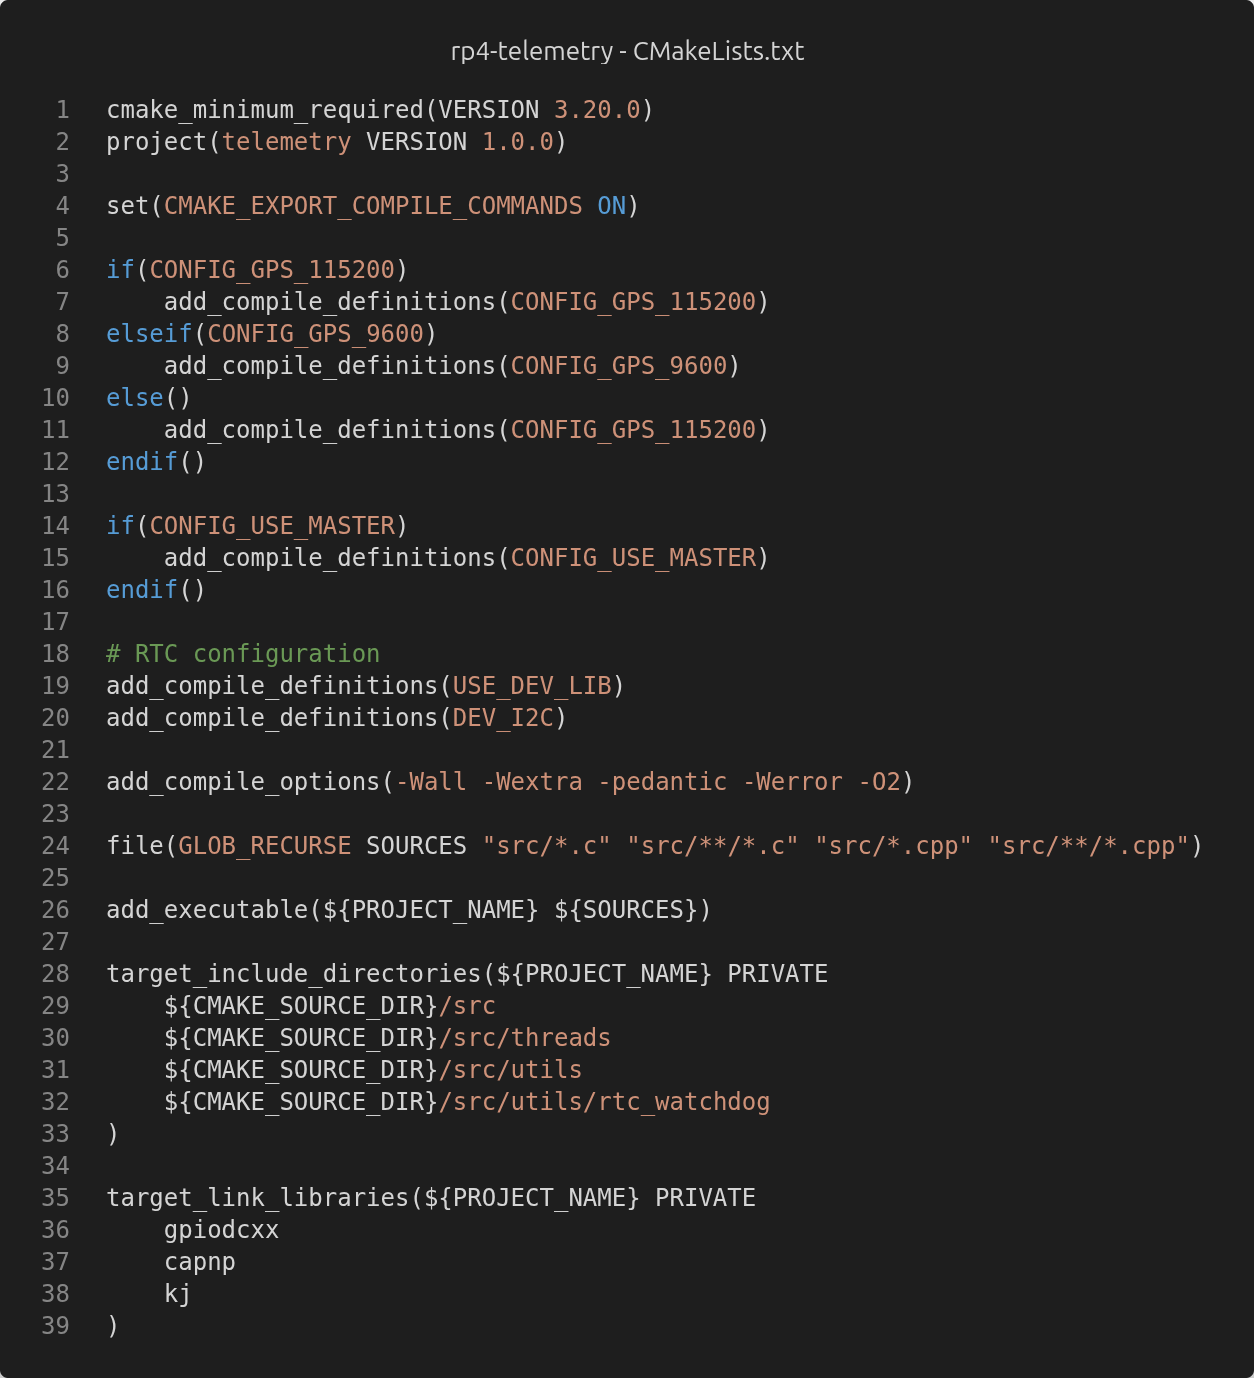
\includegraphics[width=\textwidth]{images/code/cmake.png}\par
    \caption{Binding the CAN socket}
    \label{fig:code-cmake}
\end{figure}
\FloatBarrier

In that file first the preprocessor directives used in code are set.
After that compile rules are made stricter for ensuring good practices.
Lastly all of the code and header files are added and used libraries are linked.